\documentclass[cs6size,a4paper,openany]{ctexart}

%=================== 导入配置信息 ===================
%==================== 数学符号公式 ============
\usepackage{amsmath}
\usepackage[style=1]{mdframed}
\usepackage{amsthm}
\usepackage{pdfpages}
\usepackage{amsfonts}
\usepackage{mathrsfs}
\usepackage{bm}
\usepackage{manfnt}
\usepackage{lettrine}
\def\attention{\lettrine[lines=2,lraise=0,nindent=0em]{\large\textdbend\hspace{1mm}}{}}
\usepackage{longtable}
\usepackage[toc,page]{appendix}
\usepackage{geometry}
\geometry{top=3.0cm,bottom=2.7cm,left=2.5cm,right=2.5cm} 

\usepackage{fancyhdr}
%====================清单==========================
\usepackage{enumitem}
\setlist[description]{leftmargin=\parindent,labelindent=\parindent}
%====================公式按章编号==========================
\numberwithin{equation}{section}
\numberwithin{table}{section}
\numberwithin{figure}{section}
%================= 基本格式预置 ===========================

\pagestyle{fancy}
\fancyhf{}
\fancyfoot[C]{~\zihao{5} \thepage~}
\renewcommand{\headrulewidth}{0.65pt}

% 修正：使用 \ctexset 替代已弃用的 \CTEXsetup
\ctexset{
  section = {
    format = {\centering\bfseries\zihao{3}},
    name = {第, 节},
    number = \arabic{section},
  },
  subsection = {
    format = {\bfseries\zihao{4}},
    name = {},
    number = \arabic{subsection},
  },
  subsubsection = {
    format = {\songti\zihao{-4}},
    name = {},
    number = \arabic{subsubsection},
  }
}

%================== 表格 =========================
\usepackage{makecell,rotating,multirow,diagbox}
\newcommand{\addtbl}[1]
{
	\input{table/#1}
}
%==================  图片 =========================
\newcommand{\addfig}[4][0.5]
{
  \begin{figure}[thbp!]
  \centering\includegraphics[width=#1\linewidth]{figure/#2}
  \caption{#4}
  \label{#3}
  \end{figure}
}
%================== 图形支持宏包 =========================
\usepackage{subfigure}
\usepackage{graphicx}
\usepackage{color,xcolor}
\usepackage{hyperref}
\usepackage[font=small,labelfont=bf,labelsep=space]{caption}
\captionsetup{figurewithin=section}
%==================== 源码和流程图 =====================
\newcommand{\addcode}[2][None]
{
	\lstinputlisting[language=#1]{code/#2}
}

\usepackage{listings}
\usepackage{xcolor}
\usepackage{color}
\definecolor{dkgreen}{rgb}{0,0.6,0}
\definecolor{gray}{rgb}{0.5,0.5,0.5}
\definecolor{mauve}{rgb}{0.58,0,0.82}
\definecolor{comment}{rgb}{0.56,0.64,0.68}

\lstset{
  frame=tb,
  aboveskip=3mm,
  belowskip=3mm,
  xleftmargin=2em,
  xrightmargin=2em,
  showstringspaces=false,
  keepspaces=true,
  columns=flexible,
  framerule=1pt,
  rulecolor=\color{gray!35},
  backgroundcolor=\color{gray!5},
  basicstyle={\small\ttfamily},
  numbers=none,
  numberstyle=\tiny\color{gray},
  keywordstyle=\color{blue},
  commentstyle=\color{comment},
  stringstyle=\color{dkgreen},
  breaklines=true,
  breakatwhitespace=true,
  tabsize=2,
}
%--------------------
\hypersetup{hidelinks}
\usepackage{booktabs}  
\usepackage{shorttoc}
\usepackage{tabu,tikz}
\usepackage{float}
\usepackage{multirow}

\tabcolsep=1ex
\tabulinesep=\tabcolsep
\newlength\tikzboxwidth
\newlength\tikzboxheight
\newcommand\tikzbox[1]{%
        \settowidth\tikzboxwidth{#1}%
        \settoheight\tikzboxheight{#1}%
        \begin{tikzpicture}
        \path[use as bounding box]
                (-0.5\tikzboxwidth,-0.5\tikzboxheight)rectangle
                (0.5\tikzboxwidth,0.5\tikzboxheight);
        \node[inner sep=\tabcolsep+0.5\arrayrulewidth,line width=0.5mm,draw=black]
                at(0,0){#1};
        \end{tikzpicture}%
        }

\makeatletter
\def\hlinew#1{%
  \noalign{\ifnum0=`}\fi\hrule \@height #1 \futurelet
   \reserved@a\@xhline}
   
\newcommand{\tabincell}[2]{\begin{tabular}{@{}#1@{}}#2\end{tabular}}%

\usepackage{subfigure}
\usepackage{CJK}
\usepackage{ifthen}

\newcommand{\HRule}{\rule{\linewidth}{0.5mm}}

\newtheorem{Theorem}{定理}
\newtheorem{Lemma}{引理}

\makeatletter
\@addtoreset{equation}{section}
\makeatother
\renewcommand{\theequation}{\arabic{section}.\arabic{equation}}

%-------------------------
\usepackage{pythonhighlight}
\usepackage{tikz}                    
\usepackage{tikz-3dplot}
\usetikzlibrary{shapes,arrows,positioning}

% 参考文献格式
\bibliographystyle{gbt7714-2005}

%===================  定理类环境定义 ===================
\newtheorem{example}{例}
\newtheorem{algorithm}{算法}
\newtheorem{theorem}{定理}
\newtheorem{definition}{定义}
\newtheorem{axiom}{公理}
\newtheorem{property}{性质}
\newtheorem{proposition}{命题}
\newtheorem{lemma}{引理}
\newtheorem{corollary}{推论}
\newtheorem{remark}{注解}
\newtheorem{condition}{条件}
\newtheorem{conclusion}{结论}
\newtheorem{assumption}{假设}

%==================重定义 ===================
\renewcommand{\contentsname}{目录}     
\renewcommand{\abstractname}{摘要}   
\renewcommand{\indexname}{索引}
\renewcommand{\figurename}{图}
\renewcommand{\tablename}{表}
\renewcommand{\appendixname}{附录}
\renewcommand{\proofname}{证明}
\fancyhead[C]{\zihao{5}\kaishu 实验报告：NumPy 实现全连接神经网络}

%=================== 正文开始 ===================
\begin{document}

%============== 封皮 =================
%\includepdf[page=1]{cover/cover}

%============== 目录 =================
\pagestyle{plain}
\tableofcontents
\clearpage

%============== 正文 =================
\pagenumbering{arabic}
\pagestyle{fancy}

\section{实验背景与数据集}

\subsection{实验背景}
本实验构建了一个三层全连接神经网络。
输入处理：将 MNIST 数据集中的 28×28 灰度图像展平为 784 维向量，并在输入层添加偏置项（全1列），得到 785 维输入。

网络结构：第一层全连接层将输入从 785 维映射到 256 维，后接 ReLU 激活函数；第二层全连接层将 256 维映射到 128 维，后接 ReLU 激活函数；第三层全连接层将 128 维映射到 10 维，后接 Softmax 函数输出各类别概率。

权重初始化：采用 He 初始化方法，各层权重按 $\mathrm{scale} = \sqrt{2.0 / \mathrm{input\_dim}}$ 设置随机初始值。

模块实现：将矩阵乘法、ReLU 激活、Softmax 输出、交叉熵损失分别封装为独立类，每个类均实现 forward 前向传播和 backward 反向传播方法，便于梯度计算与参数更新。
\subsection{数据集}

本实验使用 \textbf{MNIST 手写数字数据集}：

\begin{itemize}
\item 训练集：60000 张图片
\item 测试集：10000 张图片
\item 图片大小：28×28（灰度图）
\item 分类类别：10 类（数字 0–9）
\end{itemize}

\subsection{数据预处理}

\subsubsection{归一化处理}

\[
x = x / 255.0
\]

\subsubsection{标签处理}

标签转为 One-hot 编码。

\subsubsection{输入展平}

\[
28 \times 28 \rightarrow 784
\]

\subsubsection{添加偏置项}

输入层添加偏置项（+1）。

        % 实验背景
\section{实验目的}  % 原来是 \chapter

\begin{itemize}
\item 理解前向传播与反向传播的基本原理
\item 掌握全连接神经网络（MLP）的结构设计
\item 学会使用 NumPy 手动实现神经网络各模块
\end{itemize}        % 实验目的
\section{实验方法}  % 原来是 \chapter

\subsection{网络结构设计}

本实验构建了一个三层全连接神经网络。

网络结构：第一层全连接层将输入从 785 维映射到 256 维，后接 ReLU 激活函数；第二层全连接层将 256 维映射到 128 维，后接 ReLU 激活函数；第三层全连接层将 128 维映射到 10 维，后接 Softmax 函数输出各类别概率。

权重初始化：采用 He 初始化方法，各层权重按 $\mathrm{scale} = \sqrt{2.0 / \mathrm{input\_dim}}$ 设置随机初始值。

模块实现：将矩阵乘法、ReLU 激活、Softmax 输出、交叉熵损失分别封装为独立类，每个类均实现 forward 前向传播和 backward 反向传播方法，便于梯度计算与参数更新。

\subsection{网络结构示意图}

\begin{figure}[!htbp]
\centering
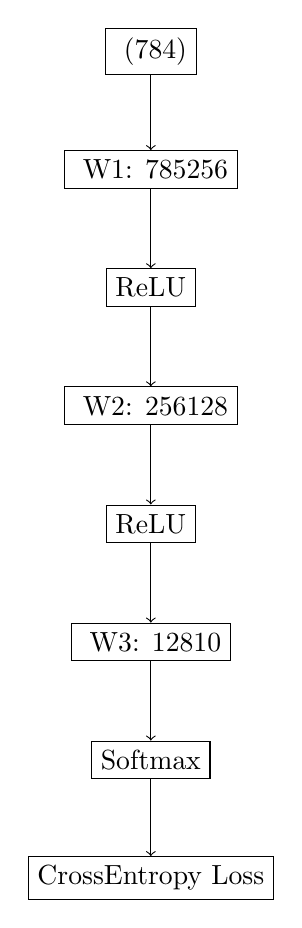
\begin{tikzpicture}[node distance=1.5cm]
\node (input) [draw, rectangle] {输入层 (784)};
\node (fc1) [draw, rectangle, below of=input] {全连接层 W1: 785×256};
\node (relu1) [draw, rectangle, below of=fc1] {ReLU};
\node (fc2) [draw, rectangle, below of=relu1] {全连接层 W2: 256×128};
\node (relu2) [draw, rectangle, below of=fc2] {ReLU};
\node (fc3) [draw, rectangle, below of=relu2] {全连接层 W3: 128×10};
\node (softmax) [draw, rectangle, below of=fc3] {Softmax};
\node (loss) [draw, rectangle, below of=softmax] {CrossEntropy Loss};

\draw[->] (input) -- (fc1);
\draw[->] (fc1) -- (relu1);
\draw[->] (relu1) -- (fc2);
\draw[->] (fc2) -- (relu2);
\draw[->] (relu2) -- (fc3);
\draw[->] (fc3) -- (softmax);
\draw[->] (softmax) -- (loss);
\end{tikzpicture}
\caption{网络结构示意图}
\label{fig:network}
\end{figure}

\subsection{各模块说明}

\subsubsection{Matmul（矩阵乘法层）}

\textbf{前向传播}：
\[
y = xW
\]

\textbf{反向传播}：
\[
\frac{\partial L}{\partial x} = \frac{\partial L}{\partial y} W^T
\]
\[
\frac{\partial L}{\partial W} = x^T \frac{\partial L}{\partial y}
\]

\subsubsection{ReLU 激活函数}

\[
f(x) = \max(0, x)
\]

\textbf{梯度}：
\[
f'(x) = 
\begin{cases} 
1 & x > 0 \\
0 & x \leq 0
\end{cases}
\]

\subsubsection{Softmax}

\[
S_i = \frac{e^{x_i}}{\sum_j e^{x_j}}
\]

\subsubsection{交叉熵损失函数}

\[
L = -\sum y \log(\hat{y})
\]

\subsection{优化方法}

\subsubsection{L2 正则化}

\[
L = L + \lambda \|W\|^2
\]

\subsubsection{动量梯度下降}

\[
v = \mu v + \eta \nabla W
\]
\[
W = W - v
\]

\subsubsection{学习率衰减}

每 10 个 epoch：
\[
lr = lr \times 0.95
\]
        % 实验方法
\section{实验结果}  % 原来是 \chapter

\subsection{训练参数}

\begin{table}[htbp]
\centering
\begin{tabular}{|l|l|}
\hline
\textbf{参数} & \textbf{取值} \\
\hline
batch\_size & 64 \\
epochs & 80 \\
初始学习率 & 0.001 \\
momentum & 0.9 \\
\hline
\end{tabular}
\caption{训练参数设置}
\label{tab:params}
\end{table}

\subsection{训练过程现象}

\begin{itemize}
\item 初期 loss 快速下降,accuracy 迅速提升至 95\%+
\item 后期收敛变慢,学习率衰减提高稳定性
\end{itemize}

\subsection{最终结果}

\begin{itemize}
\item 训练集准确率：约 99\%+
\item 测试集准确率：约 98\%+
\end{itemize}

\subsection{训练过程可视化}

训练过程中的 Loss 曲线、Accuracy 曲线和 Learning Rate 曲线如图所示。

\begin{figure}[htbp]
\centering
\begin{minipage}{0.3\textwidth}
\centering
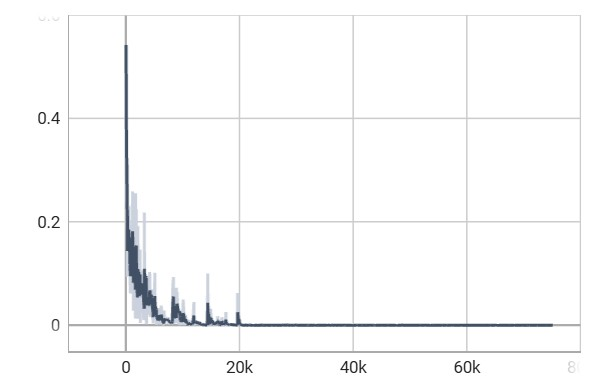
\includegraphics[width=\textwidth]{loss.jpg}
\caption{Loss 曲线}
\label{fig:loss}
\end{minipage}
\hfill
\begin{minipage}{0.3\textwidth}
\centering
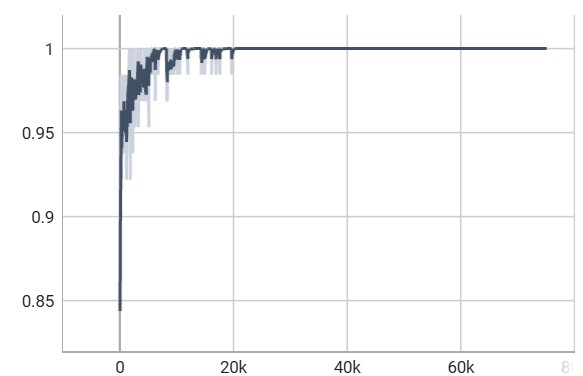
\includegraphics[width=\textwidth]{accuracy.jpg}
\caption{Accuracy 曲线}
\label{fig:accuracy}
\end{minipage}
\hfill
\begin{minipage}{0.3\textwidth}
\centering
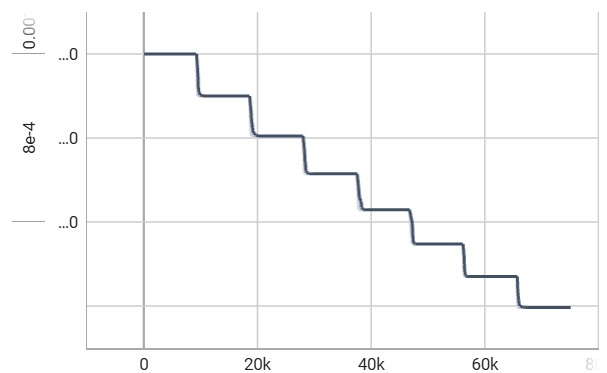
\includegraphics[width=\textwidth]{lr.jpg}
\caption{Learning Rate 曲线}
\label{fig:lr}
\end{minipage}
\label{fig:curves}
\end{figure}        % 实验结果
\section{实验分析与总结}  % 原来是 \chapter

\subsection{网络性能分析}

\begin{itemize}
\item 三层网络已能较好拟合 MNIST
\item ReLU 提高非线性表达能力
\item Softmax + 交叉熵稳定训练
\end{itemize}

\subsection{参数影响}

\begin{table}[htbp]
\centering
\begin{tabular}{|l|l|}
\hline
\textbf{参数} & \textbf{影响} \\
\hline
层数增加 & 表达能力增强但易过拟合 \\
神经元数量 & 过少欠拟合，过多计算量大 \\
学习率 & 过大震荡，过小收敛慢 \\
batch\_size & 影响稳定性与速度 \\
\hline
\end{tabular}
\caption{参数影响分析}
\label{tab:impact}
\end{table}

\subsection{优化效果}

\begin{itemize}
\item 动量：加快收敛
\item L2正则化：防止过拟合
\item 学习率衰减：提升后期稳定性
\end{itemize}

\subsection{实验总结}

本实验通过纯 NumPy 实现了一个完整的神经网络训练流程，深入理解了：

\begin{itemize}
\item 神经网络前向传播与反向传播机制
\item 各种层（Matmul、ReLU、Softmax）的作用
\item 损失函数与优化算法原理
\item 深度学习训练流程
\end{itemize}

该实验强化了对深度学习底层实现的理解，为后续使用框架（如 PyTorch）奠定了基础。        % 实验分析与总结
\input{body/appendix}        % 附录

\end{document}
